\subsection{Block Diagram}
\begin{figure}[h]
    \centering
    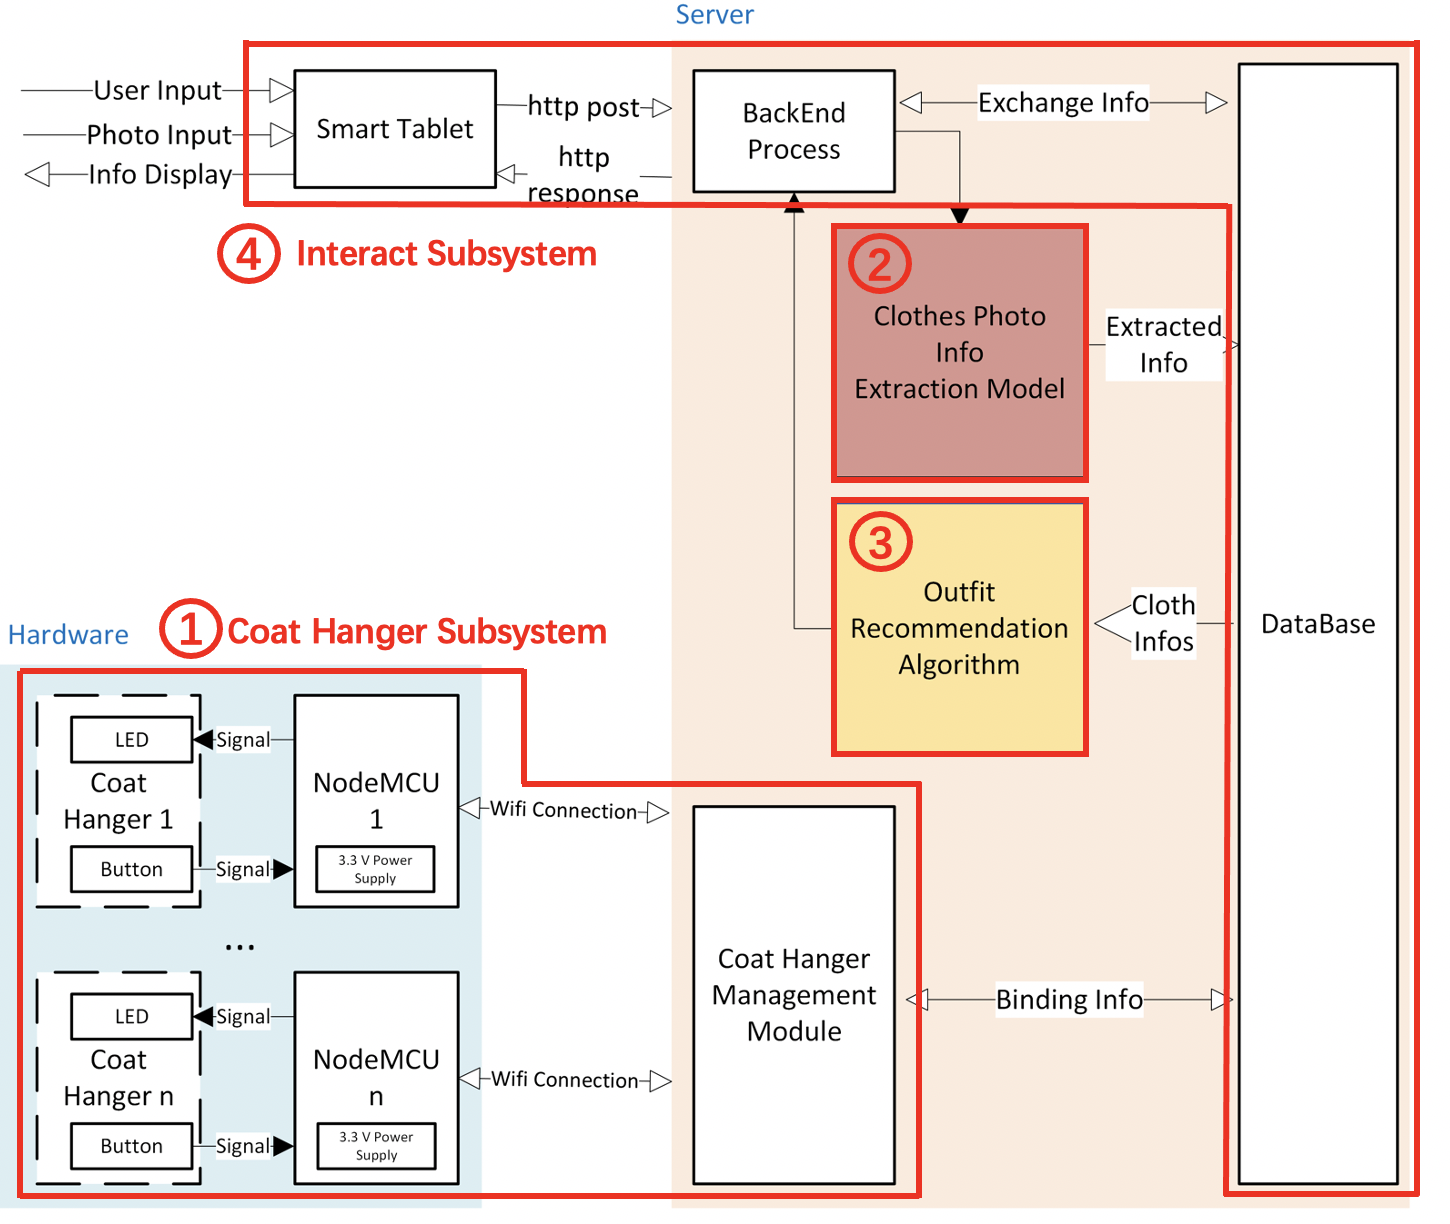
\includegraphics[width=14cm,height=13cm]{graph/block diagram.png}
    \caption{block diagram}
    \end{figure}


The block diagram gives an overview for our whole system. The blue part are hardware and the orange part are software running on the server. The system is divided into four subsystems: The interact subsystem contains the end user device (a pad), and a back end process dealing with the user's need. The back end process and the end device communicate through the http protocol and Wifi connection. And the back end process will use the Clothes Photo Info Extraction Subsystem to extract clothes info or use the Outfit Recommendation Subsystem to give user recommendations when needed. The Coat Hanger Subsystem contains the hardware part (LED, button, and NodeMCU chips which are attached on the hanger) and the Coat Hanger Management Module which is running on the server. The the Coat Hanger Management Module and the NodeMCU chip communicate through the http protocol and Wifi connection. 

\subsection{Subsystem Overview}
\subsubsection{Coat Hanger Subsystem}
The Coat Hanger Subsystem consists of a physical part (including an ordinary coat hanger and a set of circuit to control the LED light and button, and a Wi-Fi microchip to communicate with our Interact Subsystem ) and a coat hanger management algorithm running on server, as shown in the Fig. \ref{coathanger} below.
\begin{figure}[h]
   \centering
   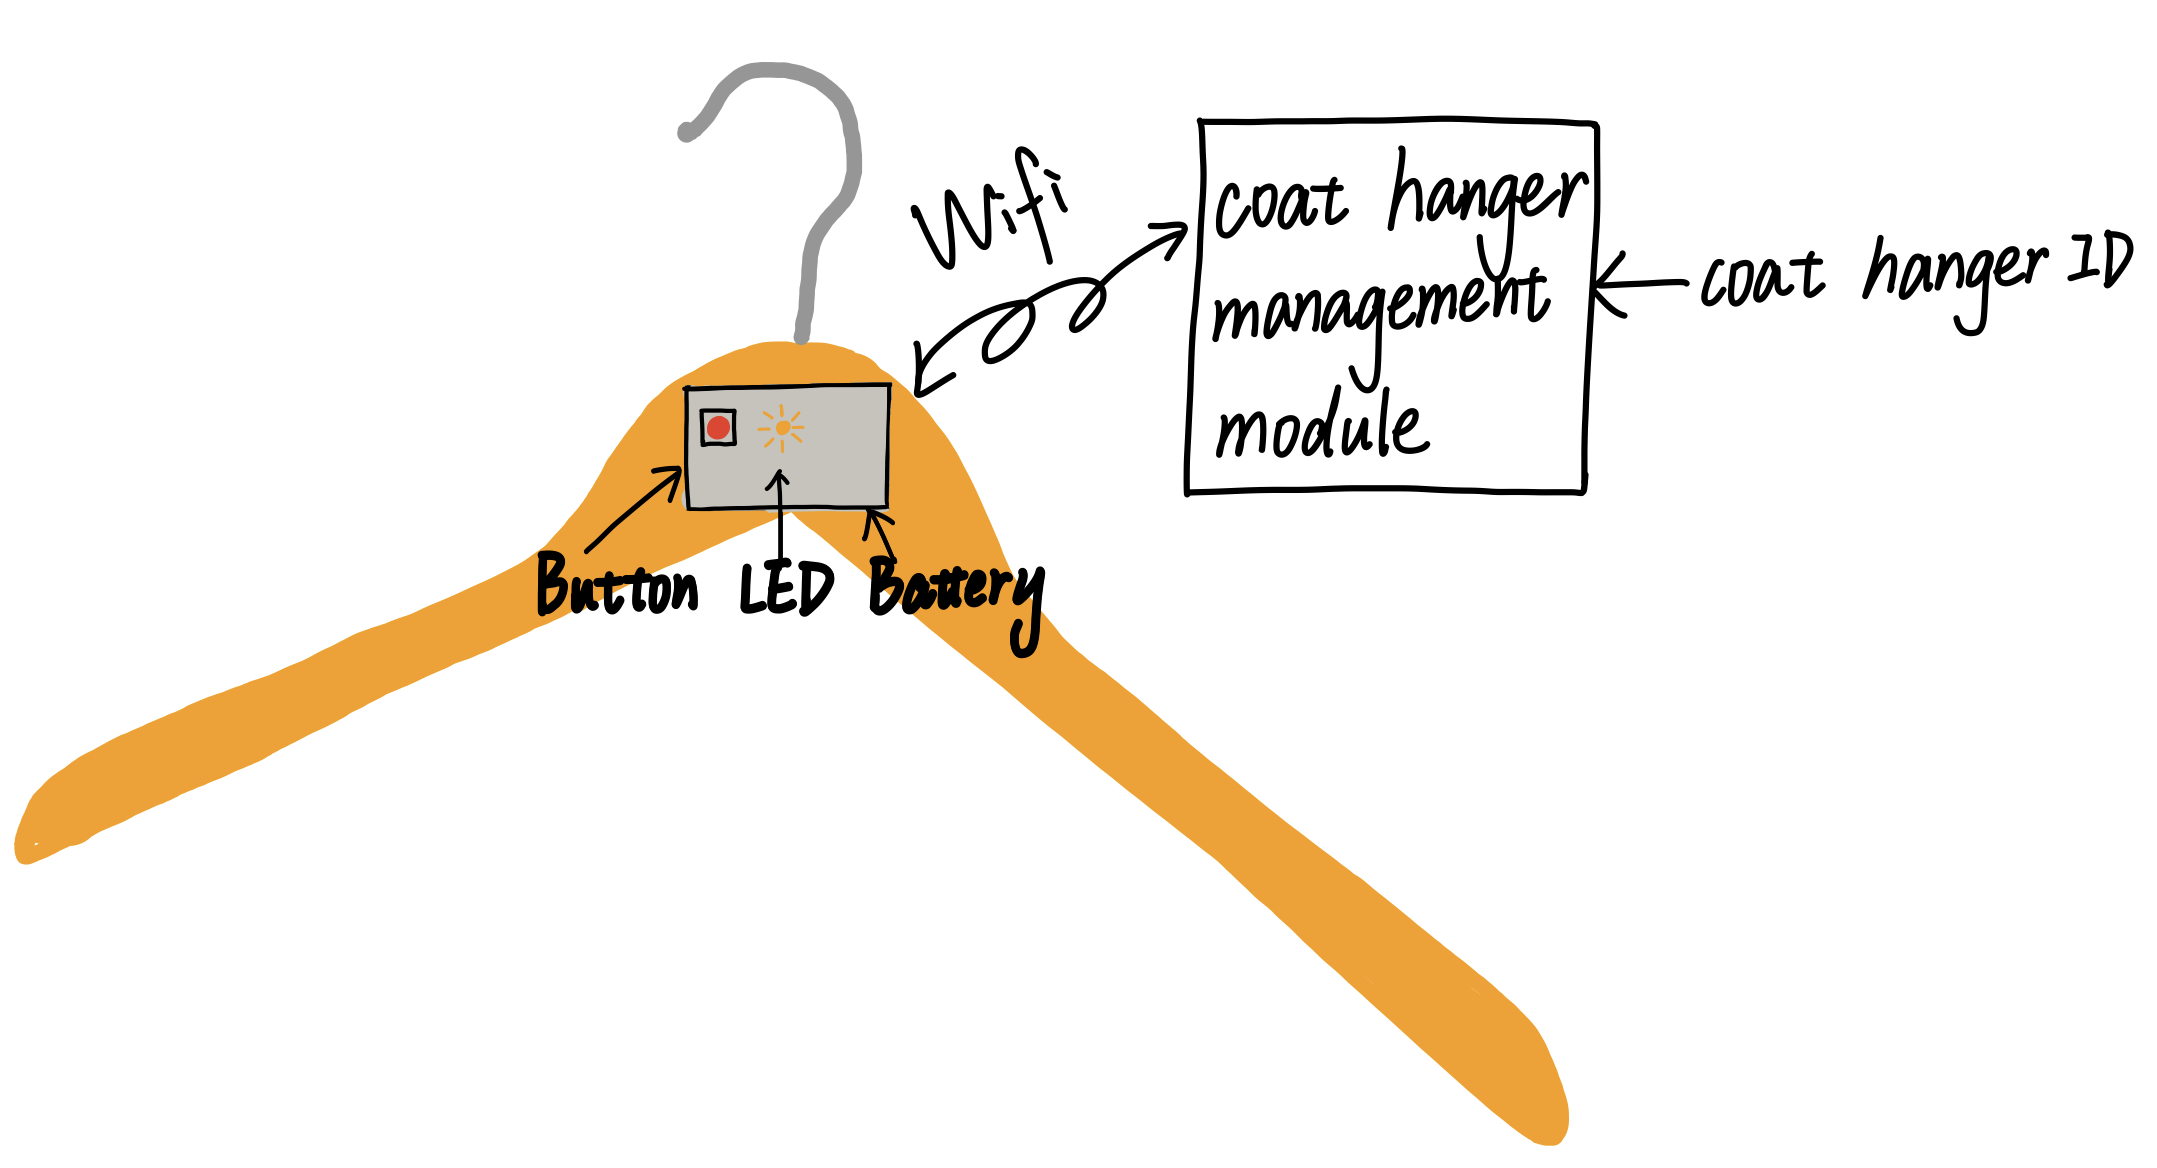
\includegraphics[width=14cm,height=8cm]{graph/Physical design for coat hanger.jpeg}
   \caption{Physical Design for the Coat Hanger}
   \label{coathanger}
   \end{figure}
 
The Coat Hanger Subsystem is designed to meet high-level requirement3 (make a user-friendly interface and allow the user easily and quickly find where the chosen clothes are). This subsystem is to help users find the recommended clothes. To be more specific, when a user gets new clothes and the photo of it is inputted, the hanger management module will automatically allocate a free coat hanger for the clothes and through the hanger information stored in the database, find the hanger to communicate with. The LED attached to this coat hanger will light to tell the user its exact location and then the user can press the button to turn off the light if he/she finishes putting his/her clothes. When the user asks the wardrobe to recommend, a certain outfit is selected by the Outfit Recommendation Subsystem, the coat hangers bound to these clothes will be called and the LED will be lit to tell the user the exact locations.  

For the circuit, Fig. \ref{circuit} below shows a detailed schematic diagram. We choose NodeMCU (CPU:ESP8266), which allows the design of single-chip devices capable of connecting via Wi-Fi, as the Wi-Fi microchip. The input voltage allowed for ESP8266 is about 3.0V-3.6V and we choose 3.3V as our power supply. At 3.3V input, when transmitting data in Wi-Fi mode, the NodeMCU has a current of about 200mA. From \textit{ESP8266 Low-Power Solutions}, a technical document by Espressif Inc. ESP8266 has three different sleep modes designed to save power as shown in Fig. \ref{esp8266}\cite{esp8266}. When it reaches deep-sleep mode, the current is about 20$\mu$A. Assuming we use a battery with a capacity of 2000mAh, we can use it for about 11.4 years in deep sleep mode. In practice, the lasting time of the Wi-Fi module depends on the actual usage of users and when the battery power is exhausted, the user can easily replace it.  

In this subsystem, we also have a hanger management algorithm running on the server. The algorithm should form a communication with the microchip equipped on coat hangers. At both clothes registering stage and recommendation stage, a request from Interact Subsystem will ask this algorithm to notify the chosen coat hanger, light the LED. After registering, this algorithm will be notified by hangers and should tell the Interact Subsystem that the task is complete. Considering the privacy issue, the target coat hanger information stored in the database is designed to be encrypted and this algorithm is the only one that holds both encryption and decryption.  

\begin{table}[h]
    \centering
    \begin{tabularx}{\textwidth}{|X|X|}
    \hline
    Requirements & Verification \\
    \hline
    1. The coat hanger can hold up to 2 kilograms (A piece of clothing is generally between 500g-2000g).
    
    2. Implement reliable communication between coats hangers and server (control delay within 2s and achieve above 90\% accuracy).
    & 
    1. Do a small load-bearing experiment. Apply two kilograms of force evenly to a coat hanger to see if it breaks.  
    
    2. Within 3 minutes, sent about 10 messages. Measure the delay time and see if the LED lit up accurately. The above tests may be carried out several times, and the delay time and accuracy should be recorded.
    \\
    \hline
    \end{tabularx}
\end{table}

\begin{figure}[h]
   \centering
   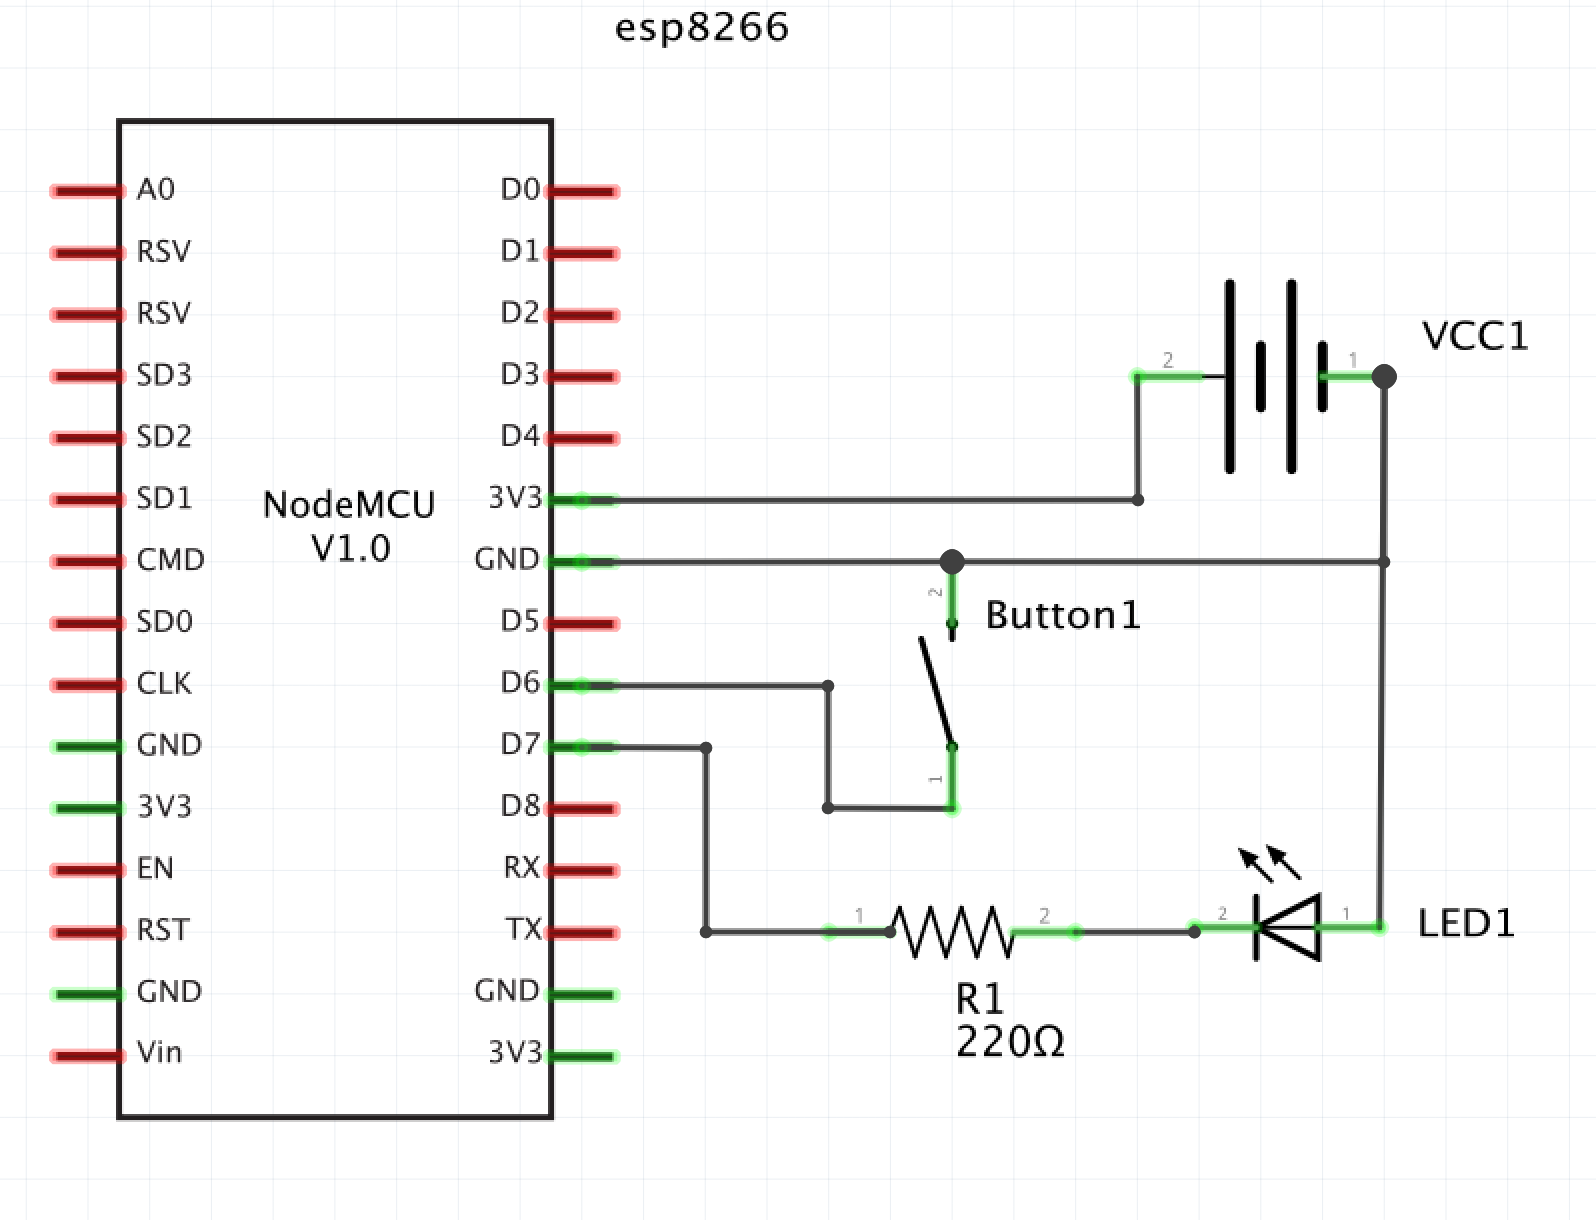
\includegraphics[width=13cm,height=10cm]{graph/The Schematic Diagram.png}
   \caption{The Schematic Diagram for Circuit}
   \label{circuit}
   \end{figure}
\begin{figure}[h]
   \centering
   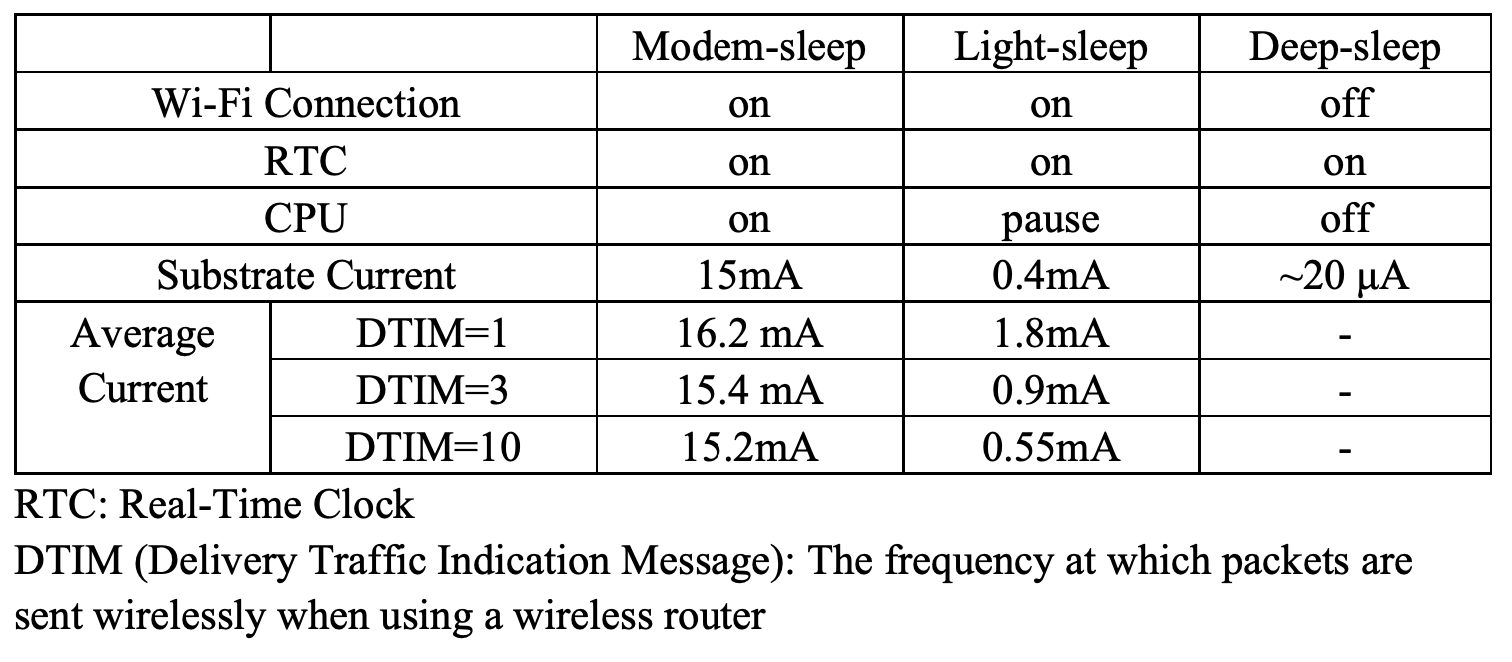
\includegraphics[width=13cm,height=6cm]{graph/esp8266 table.png}
   \caption{Three Sleep Patterns Comparison from Espressif Inc. (ESP8266 Producer)}
   \label{esp8266}
   \end{figure}

\textbf{Tolerance Analysis}   

  The power supply we choose is about 3.3V, which is generally used for our Wi-Fi module, ESP8266. The input voltage allowed for ESP8266 is about 3.0V - 3.6V, so to meet the power transmission specification, the voltage input should be within -/+0.3V (-/+9.1 \% error). There are also some errors in the impedance of the resistors and LEDs, but these small errors can be ignored because they will only influence the brightness of the led but not the operation of the circuit.
\clearpage
\subsubsection{Clothes Photo Info Extraction Subsystem}
This subsystem serves as one of our core algorithms running on the server, is designed to meet the first high-level requirement. The first task of this algorithm is to get the clothes landmark that serves as a bounding box. The second task is to predict clothes category and attributes. Every clothes is assigned with one category like jeans and several attributes such as floral, striped and knit. In the extraction stage, this algorithm will generate category and attributes for each clothes image registered by Interact Subsystem and store a unique image index with its category and attributes in our database, the category will be stored as a category index and attributes will be stored as a string of 1/0, with each one represents one attribute.  

We use FashionNet Fig. \ref{fashionnet} as our extraction model\cite{liu2016deepfashion}. The network accepts images with input dimension 224x224, the first four layers(conv1-conv4) have the same structure as VGG-16\cite{vgg}, (conv5\_pose-fc7\_pose) works as a landmark extractor, then both output from conv4 and fc7\_pose are fed into pool5\_local which serves as a landmark pooling layer, together with a global pooling achieved by conv5\_global, give the prediction of category and attributes.  

We use a large-scale data set, DeepFashion \cite{liu2016deepfashion} to train our model. This data set contains more than 280,000 images and is divided into 50 categories with 1000 attributes labeled for each image. To achieve less training cost and higher prediction accuracy, we adjust the category and attributes. The detailed strategy shows as follows: For category, the number of categories is decreased to 20 as Fig. \ref{category_change}, we delete and merge the category which contains samples less than 1000, and those serves at home such as onesie. For attributes, we delete those attributes that only be positive in less than 500 samples. Correlations between attribute pairs are computed and for two attributes with high correlation, only one should be retained. Here we define the correlation between $attribute_i$ and $attribute_j$ as $$C(i,j)=\frac{N_i\bigcap N_j}{N_i \bigcup N_j}$$, where $N_i/N_j$ denotes the number of image with $attribute_i$/$attribute_j$ is positive.  

For the training process, we will use the mmfashion \cite{mmfashion}, which is a fashion analysis toolbox developed by Multimedia Lab, CUHK. Here we also define the loss function used in our model in Fig. \ref{fashionnet}. First, a $L_2$ regression loss is used for landmarks $$L_{landmarks} = \sum_{j=1}^{|D|}\|\boldsymbol{v}_j\cdot(\hat{l}_j-l_j)\|_2^2$$ where $D$, $\hat{l}_j$, and $\boldsymbol{v}_j$ denote the number of training samples, the ground truth of the landmarks of the j-th sample and visibility of the landmark of j-th sample. Second, a 1-of-K softmax loss is used for category as $$L_{category}=\frac{1}{D}\sum_{j=1}^{D}(-\log{p_i})$$ where $D$ and ${p_i}$ denote the number of training samples and the softmax function. Third, the attribute is predicted by a weighted cross-entropy loss $$L_{attributes}=\sum_{j=1}^{|D|}(w_{pos}\cdot\boldsymbol{a}_jlog p(\boldsymbol{a}_j|\boldsymbol{x}_j)+w_{neg}\cdot(1-\boldsymbol{a}_j)log(1-p(\boldsymbol{a}_j|\boldsymbol{x}_j)))$$ where $\boldsymbol{x}_j$ and $\boldsymbol{a}_j$ denote the j-th image and attribute labels, $w_{pos}$ and $w_{neg}$ are two coefficients determined by the ratio of the number of positive and negative samples in our training set\cite{liu2016deepfashion}.  

\begin{table}[h]
    \centering
    \begin{tabularx}{\textwidth}{|X|X|}
    \hline
    Requirements & Verification \\
    \hline
    1. The prediction of top 5 category accuracy should reach 50\%.
    
    2. The prediction of top 5 Attributes recall should reach 30\%.
    & 
    1. Test the category prediction use our test set, for every one sample in our test set, if the true category label appear in the top 5 prediction, we consider the prediction as successful, otherwise failed.  
    
    2. Test the attributes prediction use our test set, the top 5 recall here define as $\frac{TP}{5}$.
    \\
    \hline
    \end{tabularx}
\end{table}

\noindent\textbf{Tolerance Analysis}  

1. One challenge here is that the accuracy of both category and attributes prediction in the clothes recognition field is still at a low level. The definition of clothing categories is vague, and the labeling of attributes varies from person to person, which makes it difficult to annotate data sets according to a certain standard, the low quality of the data set makes the model hard to learn. The consequence of poor prediction accuracy is that the wrong category and attributes will be fed into our Outfit Recommendation Subsystem and further affect recommendation performance. The solution we have to increase the accuracy here is that we give top5 or even top 10 prediction results of category and attributes to users and users can make a further correction, choose the result they agree and send to our Outfit Recommendation Subsystem so that the recommendation performance will not be affected.  

2. The second challenge is that the quality of images in our data set varies. People wearing the clothes always have different poses and face directions, which makes it hard to detect the clothes accurately, and further influences the prediction and recommendation performance. Our solution here is to suggest users upload their photos maintaining good posture so the extraction can be achieved with high accuracy.


\begin{figure}[h]
   \centering
   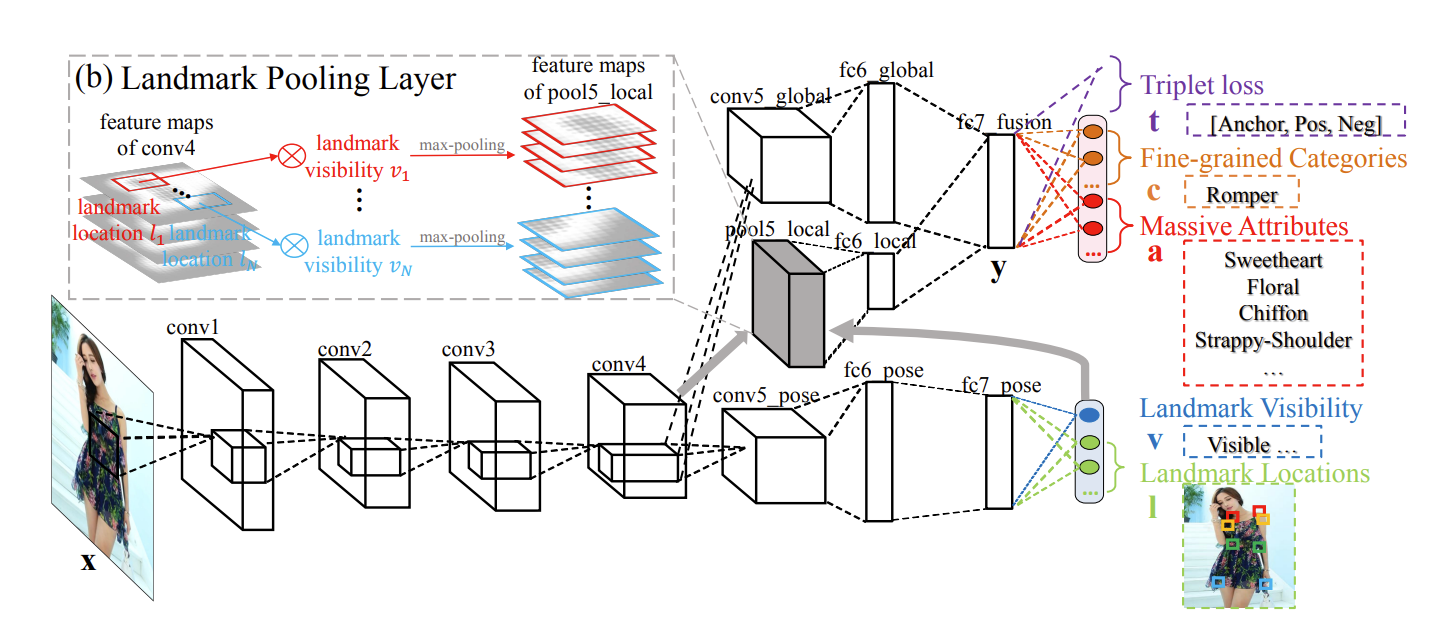
\includegraphics[width=14cm,height=9cm]{graph/FashionNet.png}
   \caption{FashionNet}
   \label{fashionnet}
   \end{figure}
   
\begin{figure}[h]
   \centering
   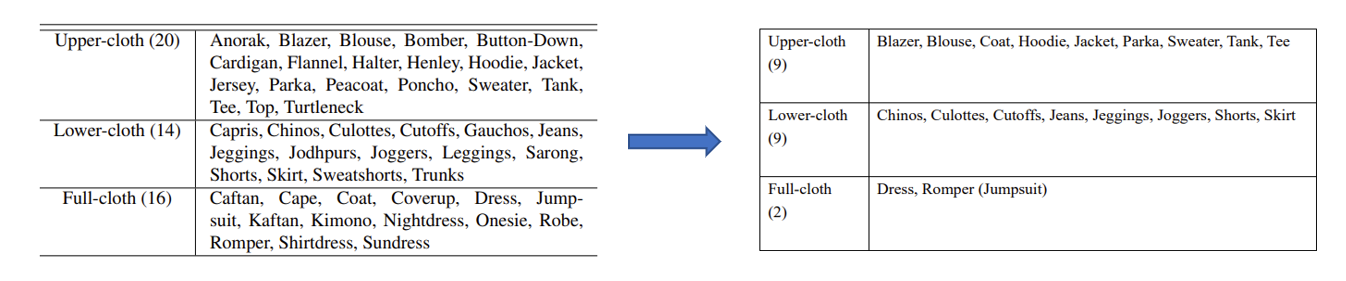
\includegraphics[width=15cm,height=5cm]{graph/category_change.png}
   \caption{Category Change}
   \label{category_change}
   \end{figure}
   
\clearpage
\subsubsection{Outfit Recommendation Subsystem}
This subsystem serves as the core algorithm to meet the second high-level requirement: give some valuable suggestion (at least 50\% of the recommendation should make sense for at least 50\% test user). It should also include some randomness to make the recommendation flexible and allow the unsatisfied user a second chance.   

The workflow of the algorithm is shown in Fig. \ref{RecommendationProcess}. The user specification input is obtained from the Interact Subsystem. Then based on the prior knowledge in the first Bayesian network, a globe combination (e.g. upper clothes + lower clothes + coat) is chosen. Then the system will decide which specific clothes to choose one by one. The first clothes (the upper cloth in Fig. \ref{RecommendationProcess}) is chosen based on the user specification and another Bayesian network, while the following clothes will be chosen based on the previous clothes just chosen. To avoid style conflict, the algorithm will tend to choose clothes similar in style to the previous one.
\begin{figure}[h]
   \centering
   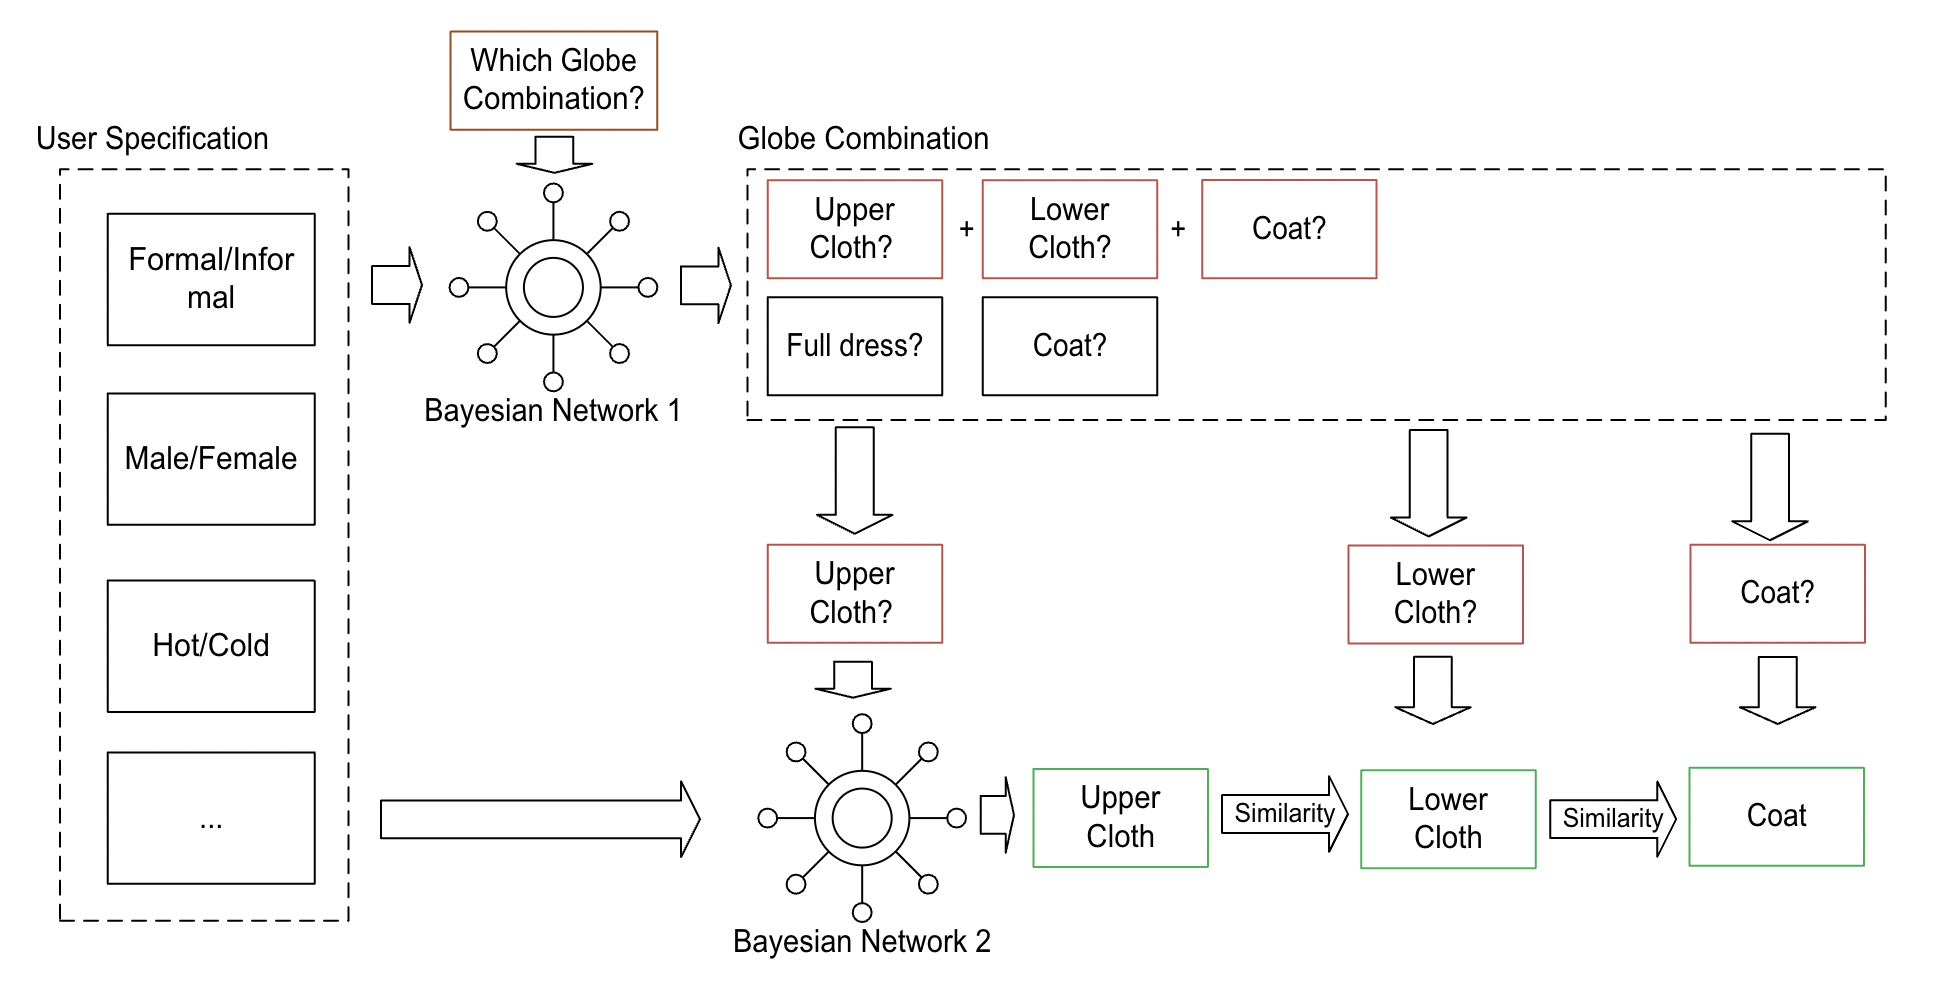
\includegraphics[width=16cm,height=10cm]{graph/recommendationDiagram.png}
   \caption{Recommendation Process}
   \label{RecommendationProcess}
   \end{figure}

The reason we use the Bayesian network in our design is that what to wear is a decision out of people's belief. Due to this subjective nature, we decided to take a subjective Bayesian view\cite{russell2010artificial} to design our algorithm. Our target is to integrate some “consensus knowledge” into our system so that the users can save themselves from spending much time and attention on that. For example, black clothes and wool materials are not recommended on hot days is a “consensus knowledge”. If our system can apply that for the user, they can spend more time and attention on their personal preference. One philosophy to keep in mind during our design process is that our system should never go too far: we should not interfere with users' preferences at any stage of the algorithm.
\begin{figure}[h]
   \centering
   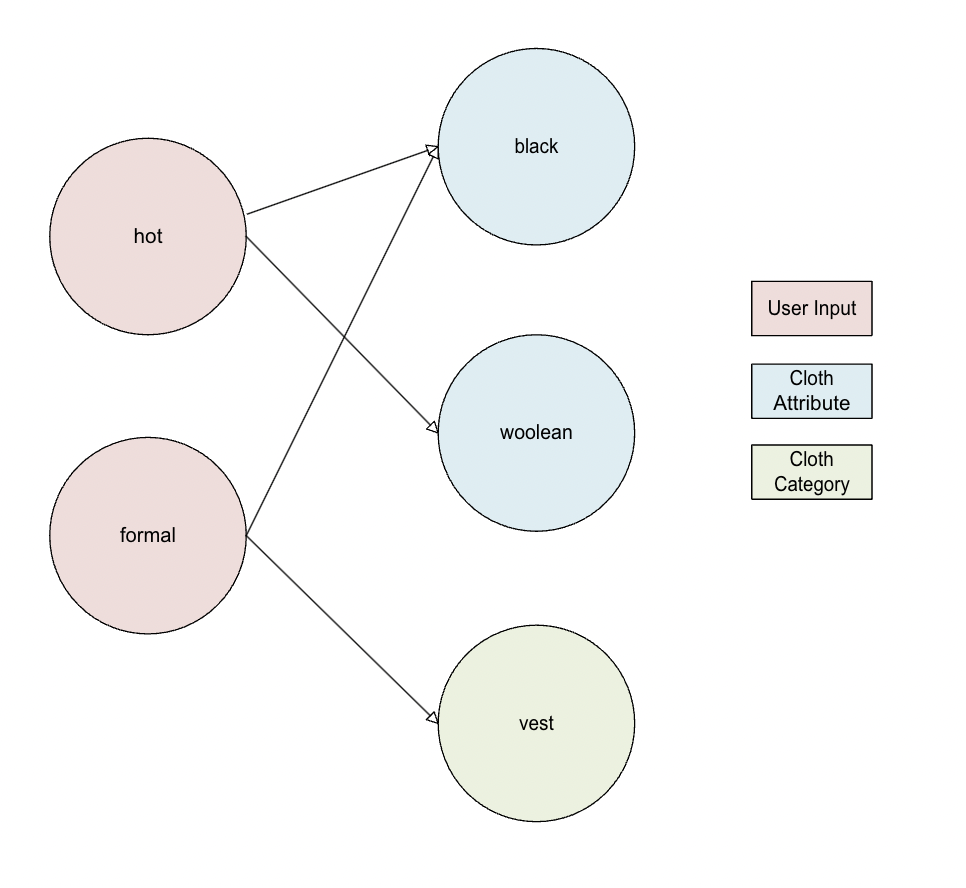
\includegraphics[width=10cm,height=7cm]{graph/BayNet.png}
   \caption{Bayesian Network Example}
   \label{BayesianNetworkExample}
   \end{figure}
   
As we can see in our example Fig. \ref{BayesianNetworkExample}, the dependence edges in the network capture those “consensus knowledge” that is widely accepted by most people (e.g. hot can affect whether to choose black cloth, formal can affect whether to choose a vest, etc.). However, the edge in the network should be far less than a complete graph. On the one hand, this choice makes the computation more efficient. On the other hand, this is a reflection of our design philosophy described before: we should not interfere with the users' preferences.
\begin{table}[h]
    \centering
    \begin{tabularx}{\textwidth}{|X|X|}
    \hline
    Requirements & Verification \\
    \hline
    1. At least 50\% of the test user should be satisfied with the recommendation result. 
    
    & 
    1. Find a group of volunteers, teach them how to use the system, then let them imagine a scenario (e.g. today is hot, you will need to go to an interview). Ask the volunteers to input their specification to the system through the user interface. Record if they find the result they want (they can ask the system to regenerate the result until they get tired with that). If more than 50\% the user are satisfied with the result in the end, we regard this subsystem as a successful implementation.

    \\
    \hline
    \end{tabularx}
\end{table}

\noindent\textbf{Tolerance Analysis} 


 1. The result of the algorithm can only be judged subjectively by the test user. And it's challenging to make sure the user is satisfied with our recommendation. To deal with that, we introduce randomness to our algorithm and allow the algorithm to be ran multiple times. If each recommendation has 30\% probability to make the user satisfied, with 10 alternative recommendations the user only have 2.82\% probability to reject all the recommendations. 

\subsubsection{Interact Subsystem}
This subsystem, which contains a database running in our server and a web tool on a smart tablet like a pad, is used for human-machine interaction. The connection between the web and our server will base on the HTTP request. This subsystem is mainly designed to satisfy the high-level requirement that users should easily and quickly find where the chosen clothes are. 
\begin{figure}[h]
   \centering
   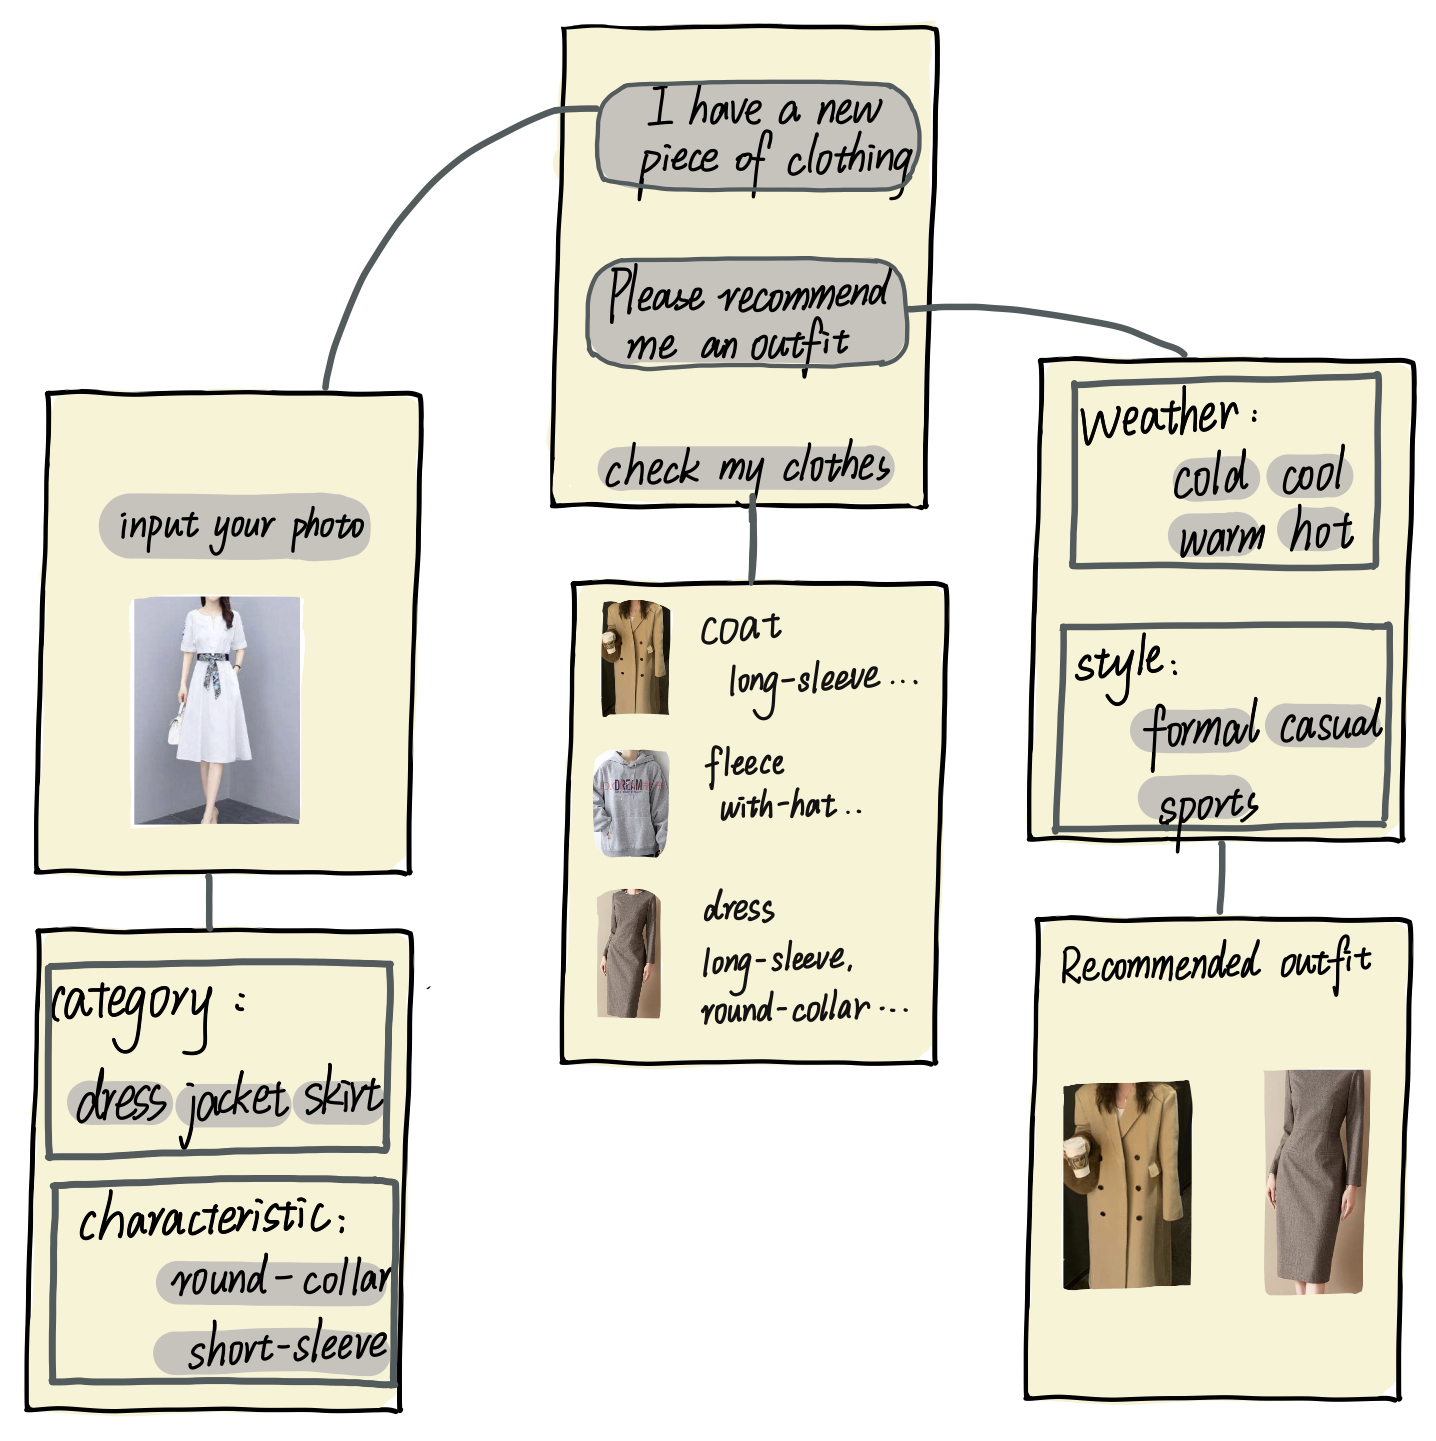
\includegraphics[width=14cm,height=11cm]{graph/Interface with users.jpeg}
   \caption{Interact with Users}
   \label{interact function}
   \end{figure}

We design the functions of this subsystem as the following three scenarios as Fig. \ref{interact function}: The first scenario is for the user to register new clothes, our web will support image upload from pad (the image should be taken beforehand and stored in pad), then the predicted clothes category and attributes by our Clothes Photo Info Extraction Subsystem will be shown to the user, the user then chooses the most conformed category and attributes, finally these data will be stored in our database. The second scenario is for the user to get a recommendation, the user needs to choose from our predefined requirements, such as weather conditions. Then, several outfits will be shown and the user can choose one they like best, then the data of chosen clothes will be stored in our database, later accessed by the algorithm in the Coat Hanger Subsystem. The third scenario is that the user can view all the registered clothes, we do not allow the user to do additions, modifications, or deletions which ensure the security and stability of the data. 
\begin{figure}[h]
   \centering
   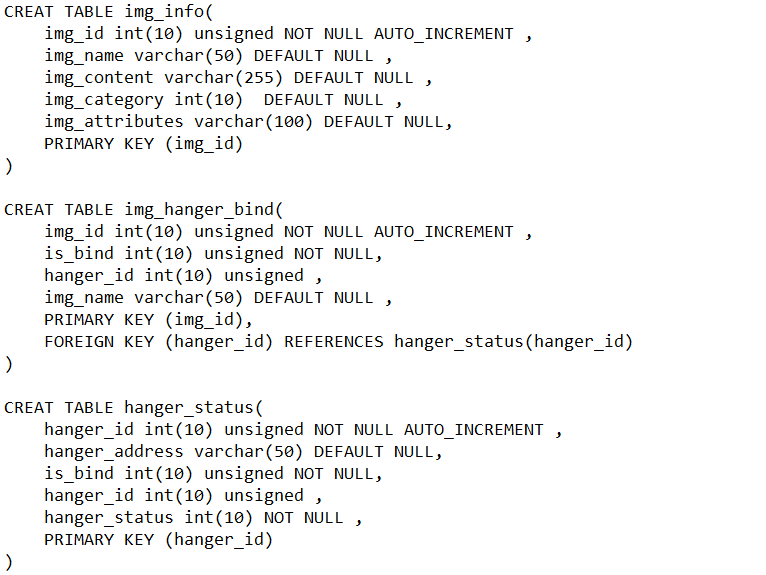
\includegraphics[width=12cm,height=8cm]{graph/db_schema.png}
   \caption{Schemas}
   \label{db_schema}
   \end{figure}


Database in this subsystem is responsible for all the data interaction, which contain data stored by the Clothes Photo Info Extraction Subsystem and data accessed by the Outfit Recommendation Subsystem. Here we define three tables in SQL, with their schemas in Fig. \ref{db_schema}. The table "img\_info" stores image with its category and attributes generated by the Outfit Recommendation Subsystem; table "img\_hanger\_bind" gives the corresponding binding of clothes and our coat hanger; table "hanger\_status" record all the coat hanger, if they have already bound, a encrypted communication address will be recorded, the algorithm in the Coat Hanger Subsystem owns the secret key which can achieve encryption and decryption.
 
We will use Django to manage the web and database, the advantage of using Django is that it turns our database into a "Model Class" after connecting and we can either use the native SQL query to access the database or work on the "Model Class" just like a python dictionary. We design four pages described as follows: the navigation page serves as the initial interface, provides users with access to the registration page, recommendation page and collection page; the registration page provides the function of image upload and prediction selection; the recommendation page provides the function of requirement selection and recommendation viewing; the collection page is for the user to manage all the registered clothes.  
\clearpage

\begin{table}[h]
    \centering
    \begin{tabularx}{\textwidth}{|X|X|}
    \hline
    Requirements & Verification \\
    \hline
    1. The web tool should be user-friendly and our users can quickly learn how to use it in 15 minutes.
    
    2. The web and database should be stable and not easy to break.
    & 
    1. Find a group of volunteers, test whether they can get familiar with both registering and recommending without any instruction.
    
    2. For web tool, test its stability using scripting tools, either detect the script and deny the access or sustain 100 visits per second; for database, test it by writing illegal data into each table, if all requests are denied, we can prove that database is also stable. 
    \\
    \hline
    \end{tabularx}
\end{table}

\noindent\textbf{Tolerance Analysis} 


 1. A database running on a server is always in danger of being hacked, which further cause User privacy leakage. To deal with possible privacy issues, we use the AES algorithm to encrypt data such as image content and hanger address. Only the algorithm in Coat Hanger Subsystem has the secret key and can decrypt.